\documentclass[a4paper, 10pt]{article}
\usepackage{amsmath}
\usepackage{amsfonts}
\usepackage{graphicx}
\usepackage[spanish]{babel}

\title{Ley de propagación de errores, justificación de la ley $\Sigma_y = J_x \Sigma_x J_x^{T}$}
\author{Joaquín Gómez}

\begin{document}
\maketitle
\pagebreak
\section{Introducción}
A la hora de medir un evento cuya entrada es una variable aleatoria $X$,
y cuya salida o variable dependiente es $Y$, otra variable aleatoria de
la cual no sabemos más que su relación con $X$, surge el siguiente
problema: ¿cómo podemos aproximar $Y$ para cualquier valor, dado que
conocemos $X$ y su relación con $Y$? Esta pregunta es trivial si se trata
de una relación totalmente lineal entre $X$ e $Y$, lo que implica
\begin{equation}
    Y=aX
\end{equation}
para un cierto número real $a$. Sin embargo, en el mundo real estas relaciones
no se cumplen de forma perfecta.

\section{Caso unidimensional}
Para este caso, donde tenemos un número de entradas que definiremos como $N=1$ y
salidas $P=1$, podemos encontrar una función $f:R\to R$ tal que
\begin{equation}
    Y = f(X)
\end{equation}

\begin{figure}[h]
    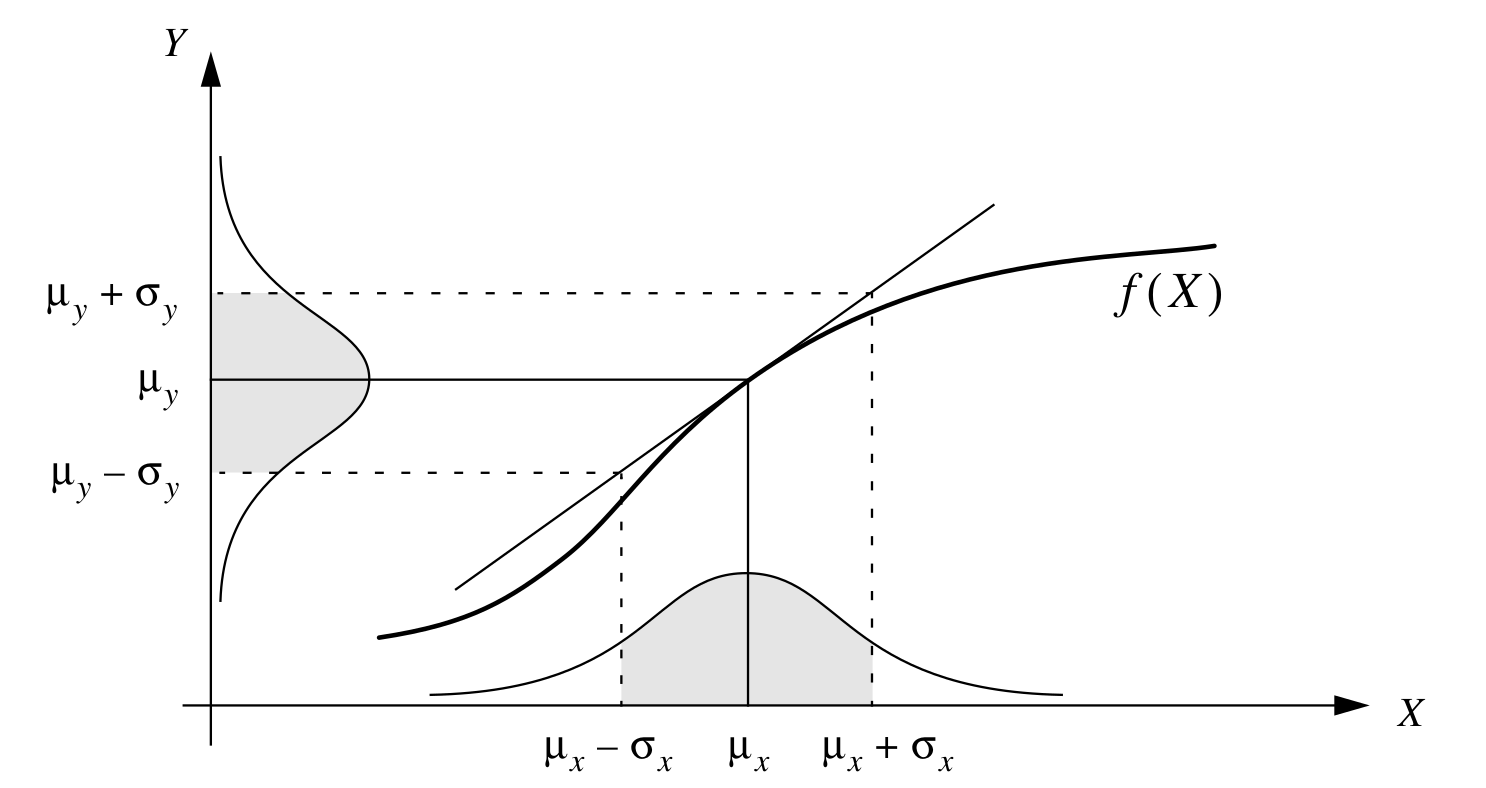
\includegraphics[width=\textwidth]{fig1.png}
    \caption{Propagación de error unidimensional}
\end{figure}

En la figura 1 se muestra un ejemplo, en el cual, a través de una aproximación
lineal, podemos determinar la distribución Gaussiana de $Y$. Para hacerlo, debemos
utilizar una aproximación de Taylor de primer orden. En este caso es
\begin{equation}
    Y = f(\mu_y) + \left. \dfrac{\partial f}{\partial X}\,\right\rvert_{X=\mu_x} \left(X-\mu_x\right)
\end{equation}
El significado del signo de ``aproximado'' es que $Y$ no va a representar el valor
\textit{real} de la función, pero puede ser una aproximación suficientemente buena, siempre
y cuando la correspondencia entre $X$ e $Y$ sea ``suficientemente lineal'' en un intervalo dado.
Se considera el intervalo $[\mu_x - \sigma_x, \mu_x + \sigma_x]$, pero también es válido,
en algunos casos, considerar $[\mu_x - 2\sigma_x, \mu_x + 2\sigma_x]$. Esto último siempre y cuando
la desviación estándar no sea muy grande.

Analicemos lo siguiente, dados los valores reales de $Y$, podríamos conocer su varianza y su media.
Supongamos que sabemos la varianza real de $Y$, dada como $\sigma^{2}_0$ y su media $\mu_0$. Ahora,
si suponemos
\begin{equation}
    \begin{split}
        \sigma^{2}_o \approx \sigma^{2}_y \\
        \mu_o \approx \mu_y \\
    \end{split}
\end{equation}
entonces podemos utilizar la aproximación para encontrar
\begin{equation}
    \begin{split}
        &\mu_y = f(\mu_x)\\
        &\sigma_y = \left.\dfrac{\partial f}{\partial X}\right\rvert_{X=\mu_x} \sigma_x
    \end{split}
\end{equation}
En una situación real, debemos inferir los valores de $\mu_x$ y $\sigma_x$, o intentar
adivinarlos. En esta situación, se tiene que dar que nuestro valor de muestra $X = x^{*}$ sea cercano
a $E[X]$. Basándonos en este principio, podemos a su vez intentar hallar un valor aproximado para
$s_x^{*}$, que deberá ser cercano a $E\left[(X-\mu_x)^{2}\right]^{1/2}$. Si cumplimos ambas condiciones,
obtendremos un valor de $y^{*}$ no tan alejado de $E[Y]$, y una desviación estándar $s_y^{*}$ también
suficientemente cerca de $E\left[(Y-\mu_y)^{2}\right]^{1/2}$.

Matemáticamente, dada una muestra $X = x^{*} \approx E[X]$ y un valor inferido $s_x^{*} \approx \sigma_x$,
tenemos que, la aproximación $Y = y^{*}$ y $s_y^{*}$ cumplen
\begin{equation}
    \begin{split}
        &y^{*} \approx E[Y] \\
        &s_y^{*} \approx \sigma_y
    \end{split}
\end{equation}

En este caso, lo que se intenta decir es que las medidas reales que nosotros tomemos, pueden ser similares
a las que resulten de nuestra aproximación, siempre y cuando se cumpla que los valores de entrada sean representativos.
En otras palabras, si tomamos una muestra y corresponde a un valor cercano al promedio, entonces debería cumplirse
que la salida de nuestro sistema también sea cercana a su promedio.

\section{Sistema con varias entradas y una salida}
Para este caso, tendremos una serie de $N = n$ entradas $X_1,X_2,\dots,X_n$ y $P = 1$ salida.
La función $f:R^{n} \to R$ es un campo escalar y nos da la relación
\begin{equation}
    f(X_1,X_2,\dots,X_n) = Y
\end{equation}
Nuevamente, utilizaremos la aproximación de Taylor de primer orden
\begin{equation}
    \begin{split}
        Y = f(\mu_x^{(1)}, \mu_x^{(2)},\dots,\mu_x^{(n)}) +
        \sum_{i=1}^{n}{\dfrac{\partial f}{\partial X_i}
        \left(\mu_x^{(1)}, \mu_x^{(2)},\dots,\mu_x^{(n)}\right)(X_i-\mu^{(i)}_x)}
    \end{split}
\end{equation}
(nótese que la derivada parcial está aplicada en el vector $\mu_x$). Así, podemos encontrar la
media y desviación estándar de $Y$, definiremos dos variables, que son
$a_0 = f(\mu_x^{(1)}, \mu_x^{(2)},\dots,\mu_x^{(n)})$ y $a_i = \dfrac{\partial f}{\partial X_i}\left(\mu_x^{(1)}, \mu_x^{(2)},\dots,\mu_x^{(n)}\right)$,
de forma que obtenemos
\begin{equation}
    \begin{split}
        \mu_y & = E\left[Y\right] \\
        &=E\left[a_0 + \sum_{i}^{}{a_i(X_i-\mu_x^{(i)})}\right] \\
        &=E[a_0] + E\left[\sum_{i}^{}{a_i(X_i-\mu_x^{(i)})}\right] \\
        &=a_0 + \sum_{i}^{}a_iE\left[{X_i}\right] - \sum_{i}^{}a_iE\left[\mu_x^{(i)}\right] \\
        &=a_0 + \sum_{i}^{}a_i\mu_x^{(i)} - \sum_{i}^{}a_i\mu_x^{(i)} \\
        &=a_0 \\[2em]
    \end{split}
\end{equation}
Para hallar la desviación estándar, el camino es más largo, para ello utilizamos la varianza
\begin{equation}
    \begin{split}
        \sigma_y^{2} &= E\left[(Y-\mu_y)^{2}\right] \\
        &=E\left[\left(\sum_{i}^{}{a_i(X_i-\mu_x^{(i)})}\right)^{2}\right] \\
        &=E\left[\sum_{i}^{}{a_i(X_i-\mu_x^{(i)})} \sum_{j}^{}{a_j(X_j-\mu_x^{(j)})}\right] \\
        &=E\left[\sum_{i}^{}{a_i^{2}(X_i-\mu_x^{(i)})^{2}}+\mathop{\sum\sum}_{i\neq j}{a_i a_j (X_i-\mu_x^{(i)})(X_j-\mu_x^{(j)})}\right] \\
        &=E\left[\sum_{i}^{}{a_i^{2}(X_i-\mu_x^{(i)})^{2}}\right]+E\left[\mathop{\sum\sum}_{i\neq j}{a_i a_j (X_i-\mu_x^{(i)})(X_j-\mu_x^{(j)})}\right] \\
        &=\sum_{i}^{}a_i^{2}E\left[{(X_i-\mu_x^{(i)})^{2}}\right]+\mathop{\sum\sum}_{i\neq j}a_i a_jE\left[{ (X_i-\mu_x^{(i)})(X_j-\mu_x^{(j)})}\right] \\
        &=\sum_{i}^{}a_i^{2}\textnormal{Var}(X_i)+\mathop{\sum\sum}_{i\neq j} a_i a_j\textnormal{Cov}(X_i, X_j) \\
        &=\sum_{i}^{}\left(\left.\dfrac{\partial f}{\partial X_i}\right\rvert_{X=\mu_x}\right)^{2}\textnormal{Var}(X)+\mathop{\sum\sum}_{i\neq j} \left.\dfrac{\partial f}{\partial X_i}\right\rvert_{X=\mu_x} \left.\dfrac{\partial f}{\partial X_j}\right\rvert_{X=\mu_x}\textnormal{Cov}(X_i, X_j) \\
        &=\sum_{i}^{}\left(\left.\dfrac{\partial f}{\partial X_i}\right\rvert_{X=\mu_x}\right)^{2}\sigma^{2}_x+\mathop{\sum\sum}_{i\neq j} \left.\dfrac{\partial f}{\partial X_i}\right\rvert_{X=\mu_x} \left.\dfrac{\partial f}{\partial X_j}\right\rvert_{X=\mu_x}\Sigma^{2}_{ij} \\
    \end{split}
\end{equation}
Entonces, la desviación estándar es
\begin{equation}
    \sigma_y=\sqrt{\sum_{i}^{}\left(\left.\dfrac{\partial f}{\partial X_i}\right\rvert_{X=\mu_x}\right)^{2}\sigma^{2}_x+\mathop{\sum\sum}_{i\neq j} \left.\dfrac{\partial f}{\partial X_i}\right\rvert_{X=\mu_x} \left.\dfrac{\partial f}{\partial X_j}\right\rvert_{X=\mu_x}\Sigma^{2}_{ij}}
\end{equation}
Si las variables independientes no están relacionadas entre sí, $\textnormal{Cov}(X_i, X_j) = 0$ para $j\neq i$,
entonces la fórmula se resume en
\begin{equation}
    \sigma_y^{2} = \sum_{i}^{}\left(\dfrac{\partial f}{\partial X_i}\right)^{2}\sigma^{2}_x
\end{equation}
Donde suponemos que aplicamos la derivada parcial en un punto fijo, que será en este caso, la media $u_x$.
Omitimos esto para abreviar la fórmula y evitar así demasiada sintaxis.

\section{Sistema con múltiples entradas y salidas}
Este caso es una generalización del caso anterior, tomamos las ideas que ya conocemos, para encontrar la fórmula
más recurrente para la propagación de errores, que es
\begin{equation}
    \Sigma_y = F_x \Sigma_x F_x^{T}
\end{equation}
¿Cómo encaramos el problema? Antes que nada, definiremos la función que relaciona una serie de entradas $X_1,X_2,\dots,X_n$ a una serie de salidas $f_1,f_2,\dots,f_p$.
Tendremos que el sistema tiene $N=n$ y $P=p$ entradas y salidas respectivamente. De forma que la función que lo representa es $f:R^{n} \to R^{p}$ un campo vectorial, así
\begin{equation}
    \begin{cases}
        Y_1 = f_1(X_1,X_2,\dots,X_n) \\
        Y_2 = f_2(X_1,X_2,\dots,X_n) \\
        \vdots                       \\
        Y_p = f_p(X_1,X_2,\dots,X_n)
    \end{cases}
\end{equation}
Para esta sección, definiremos $Y=\left(Y_1,Y_2,\dots,Y_n\right)$.
Buscaremos una fórmula para la aproximación de Taylor de primer orden, como vimos en la sección anterior
\begin{equation}
    Y_i = f_i(X_1,X_2,\dots,X_n) + \sum_{k=1}^{n}{\dfrac{\partial f_i}{\partial X_k}
    \left(X_1,X_2,\dots,X_n\right)\left(X_k - \mu_{x}^{k}\right)}
\end{equation}
Si observamos bien, podemos representar al segundo miembro del lado derecho de la ecuación como
el producto escalar $\nabla f_i \cdot (X-\mu_x)$
\begin{equation}
    Y_i = f_i(X_1,X_2,\dots,X_n) + \nabla f_i \cdot (X-\mu_x)
\end{equation}
Asímismo, podemos escribir $Y$ como una suma de dos vectores, donde $X=\left(X_1\, X_2\, \cdots\, X_n\right)$ y
$\mu_x = \left(\mu_x^{(1)}\,\mu_x^{(2)}\,\cdots\, \mu_x^{(n)}\right)$
\begin{equation}
    Y = \begin{bmatrix}
        f_1(\mu_x) \\
        f_2(\mu_x) \\
        \vdots     \\
        f_p(\mu_x)
    \end{bmatrix} +
    \begin{bmatrix}
        \nabla f_1\left(\mu_x\right) \cdot (X-\mu_x) \\
        \nabla f_2\left(\mu_x\right) \cdot (X-\mu_x) \\
        \vdots                                       \\
        \nabla f_p\left(\mu_x\right) \cdot (X-\mu_x)
    \end{bmatrix}
\end{equation}
Si separamos el vector con los gradientes $\nabla f_i$, y los expandimos, obtendríamos la matriz Jacobiana
\begin{equation}
    J_x(X) = \begin{bmatrix}
        \nabla f_1\left(\mu_x\right) \\
        \nabla f_2\left(\mu_x\right) \\
        \vdots                       \\
        \nabla f_p\left(\mu_x\right)
    \end{bmatrix} = \begin{bmatrix}
        \dfrac{\partial f_1(X)}{\partial X_1} & \cdots & \dfrac{\partial f_1(X)}{\partial X_n} \\
        \vdots                                & \ddots & \vdots                                \\
        \dfrac{\partial f_p(X)}{\partial X_1} & \cdots & \dfrac{\partial f_p(X)}{\partial X_n} \\
    \end{bmatrix}
\end{equation}
de forma tal que, podemos reescribir (17) como
\begin{equation}
    Y = f(\mu_x) + J_x(\mu_x)\cdot (X-\mu_x)
\end{equation}

Debemos encontrar la covarianza de $Y$, para ello, sin perder generalidad, buscamos el elemento
en la posición $ij$ en la matriz de covarianza $\Sigma_y$ y el elemento $i$ en el vector $\mu_y$.
Definimos $a_{i0} = f_i(\mu_x^{(1)}, \mu_x^{(2)},\dots,\mu_x^{(n)})$ y $a_{ij} = \dfrac{\partial f_i}{\partial X_j}(\mu_x^{(1)}, \mu_x^{(2)}, \dots,\mu_x^{(n)})$
\begin{equation}
    \begin{split}
        \mu_y^{(i)} &= E\left[Y_i\right] \\
        &=E\left[a_{i0} + \sum_{j}{a_{ij}(X_j-\mu_x^{(j)})}\right] \\
        &=E\left[a_{i0}\right] + E\left[\sum_{j}{a_{ij}X_j}\right] - E\left[\sum_{j}{a_{ij}\mu_x^{(j)}}\right] \\
        &=a_{i0} + \sum_{j}a_{ij}E\left[{X_j}\right] - \sum_{j}a_{ij}\mu_x^{(j)} \\
        &=a_{i0} + \sum_{j}a_{ij}\mu_x^{(j)} - \sum_{j}a_{ij}\mu_x^{(j)} \\
        &=a_{i0} \\
    \end{split}
\end{equation}
\begin{equation}
    \begin{split}
        \Sigma_y^{(ij)} &= \textnormal{Cov}(Y_i, Y_j) \\
        &=E\left[(Y_i-\mu_y^{(i)})(Y_j-\mu_y^{(j)})\right] \\
        &=E\left[\sum_{k}{a_{ik}(X_k-\mu_x^{(k)})}\sum_{l}{a_{jl}(X_l-\mu_x^{(l)})}\right] \\
        &=E\left[\sum_{k}{a_{ik}a_{jk}(X_k-\mu_x^{(k)})^{2}} + \mathop{\sum\sum}_{l\neq k}{a_{jl}a_{ik}(X_l-\mu_x^{(l)})(X_k-\mu_x^{(k)})}\right] \\
        &=E\left[\sum_{k}{a_{ik}a_{jk}(X_k-\mu_x^{(k)})^{2}}\right]+E\left[\mathop{\sum\sum}_{l\neq k}{a_{jl}a_{ik}(X_l-\mu_x^{(l)})(X_k-\mu_x^{(k)})}\right] \\
        &=\sum_{k}a_{ik}a_{jk}E\left[{(X_k-\mu_x^{(k)})^{2}}\right]+\mathop{\sum\sum}_{l\neq k}a_{jl}a_{ik}E\left[{(X_l-\mu_x^{(l)})(X_k-\mu_x^{(k)})}\right] \\
        &=\sum_{k}a_{ik}a_{jk}\Sigma_x^{kk}+\mathop{\sum\sum}_{l\neq k}a_{jl}a_{ik}\Sigma_x^{(lk)} \\
        &=\mathop{\sum\sum}_{k,l}{a_{jl}a_{ik}\Sigma_x^{(lk)}} \\
        &=\mathop{\sum\sum}_{k,l}{\dfrac{\partial f_j}{\partial X_l} \dfrac{\partial f_i}{\partial X_k}\Sigma_x^{(lk)}}
    \end{split}
\end{equation}
Recordemos que la matriz de covarianza de $X$ está dada por
\begin{equation}
    \Sigma_x = \begin{bmatrix}
        \Sigma_x^{(11)} & \Sigma_x^{(12)} & \cdots & \Sigma_x^{(1n)}   \\
        \Sigma_x^{(21)} & \Sigma_x^{(22)} & \cdots & \Sigma_x^{(2n)}   \\
        \vdots          & \vdots          & \ddots & \vdots            \\
        \Sigma_x^{(n1)} & \Sigma_x^{(n2)} & \cdots & \Sigma_x^{(22)} & \\
    \end{bmatrix}
\end{equation}
La expresión (21) es lo mismo que
\begin{equation}
    \begin{split}
        \Sigma_y^{(ij)} &= \nabla f_i \cdot \Sigma_x \cdot \nabla f_j \\[1em]
        &=\begin{bmatrix}
            \dfrac{\partial f_i}{\partial X_1} \\
            \vdots                             \\
            \dfrac{\partial f_i}{\partial X_n} \\
        \end{bmatrix}
        \cdot
        \begin{bmatrix}
            \Sigma_x^{(11)} & \Sigma_x^{(12)} & \cdots & \Sigma_x^{(1n)}   \\
            \Sigma_x^{(21)} & \Sigma_x^{(22)} & \cdots & \Sigma_x^{(2n)}   \\
            \vdots          & \vdots          & \ddots & \vdots            \\
            \Sigma_x^{(n1)} & \Sigma_x^{(n2)} & \cdots & \Sigma_x^{(22)} & \\
        \end{bmatrix}
        \cdot
        \begin{bmatrix}
            \dfrac{\partial f_j}{\partial X_1} \\
            \vdots                             \\
            \dfrac{\partial f_j}{\partial X_n} \\
        \end{bmatrix}
        \\[1em]
        &=\begin{bmatrix}
            \sum_{k} {\frac{\partial f_i}{\partial X_k}\Sigma_x^{(k1)}}\\
            \sum_{k} {\frac{\partial f_i}{\partial X_k}\Sigma_x^{(k2)}}\\
            \vdots \\
            \sum_{k} {\frac{\partial f_i}{\partial X_k}\Sigma_x^{(kn)}}        
        \end{bmatrix}\cdot
        \begin{bmatrix}
            \dfrac{\partial f_j}{\partial X_1} \\
            \vdots                             \\
            \dfrac{\partial f_j}{\partial X_n} \\
        \end{bmatrix}\\[1em]
        &=\sum_{k} {\frac{\partial f_i}{\partial X_k}\frac{\partial f_j}{\partial X_1}\Sigma_x^{(k1)}} + \cdots + \sum_{k} {\frac{\partial f_i}{\partial X_k}\frac{\partial f_j}{\partial X_n}\Sigma_x^{(kn)}}\\[1em]
        &=\sum_{k}\sum_{l}{\frac{\partial f_i}{\partial X_k}\frac{\partial f_j}{\partial X_l}\Sigma_x^{(kl)}}
    \end{split}
\end{equation}
Si generalizamos la expresión, obtenemos la ecuación de la ley de propagación de errores
\begin{equation}
    \Sigma_y = J_x \Sigma_x J_x^{T}
\end{equation}
En nuestro caso, aplicamos $\mu_x$ en la matriz Jacobiana, es decir
\begin{equation}
    \Sigma_y = J_x(\mu_x) \Sigma_x \left[J_x(\mu_x)\right]^{T}
\end{equation}
La fórmula (24) expresa un cambio de base (lineal) aplicado a la matriz de covarianza de $X$. Básicamente, estamos transformando la covarianza de $X$ a
través de su relación con $Y$, esta relación está dada por la matriz Jacobiana, ya que expresa la tasa de cambio de cada salida $Y_i$ con respecto a sus
variables $X_j$. El significado intuitivo es el mismo que en el caso unidimensional.

\end{document}